\documentclass{article}
\usepackage{graphicx}
\usepackage[margin=1.5cm]{geometry}
<<<<<<< HEAD
\usepackage{amsmath,amsfonts}
=======
\usepackage{amsmath}
>>>>>>> 984fdb315abd4b8f89026c773978005f8f0c3ed8

\begin{document}

\title{Monday Reading Assessment: Unit 2, Ohm's Law and Batteries, Kirchhoff's Rules}
\author{Prof. Jordan C. Hanson}

\maketitle

\section{Memory Bank}

\begin{itemize}
<<<<<<< HEAD
\item $i_{\rm in} = i_{\rm out}$ ... Kirchhoff's junction rule.
\item $\epsilon_1 + \epsilon_2 + \epsilon_3 + ... = 0$ ... Kirchhoff's loop rule.
\end{itemize}

\section{Kirchhoff's Rules Tutorial}

\begin{enumerate}
\item Recall the Kirchhoff's Rules tutorial video 1.  We solved for the current $i_1$ in Fig. \ref{fig:dura}. (a) What is $i_2$? Once you find $i_2$, find $i_3$ using the junction rule.  What does the sign of $i_3$ tell us about the lower battery? (b) Suppose the emf of battery 2 was raised to $\epsilon_2 = 12$ V, and we observe that $i_1 = 1.2$A and $i_2 = 1.2$A. What is $i_3$?
\begin{figure}[ht]
\centering
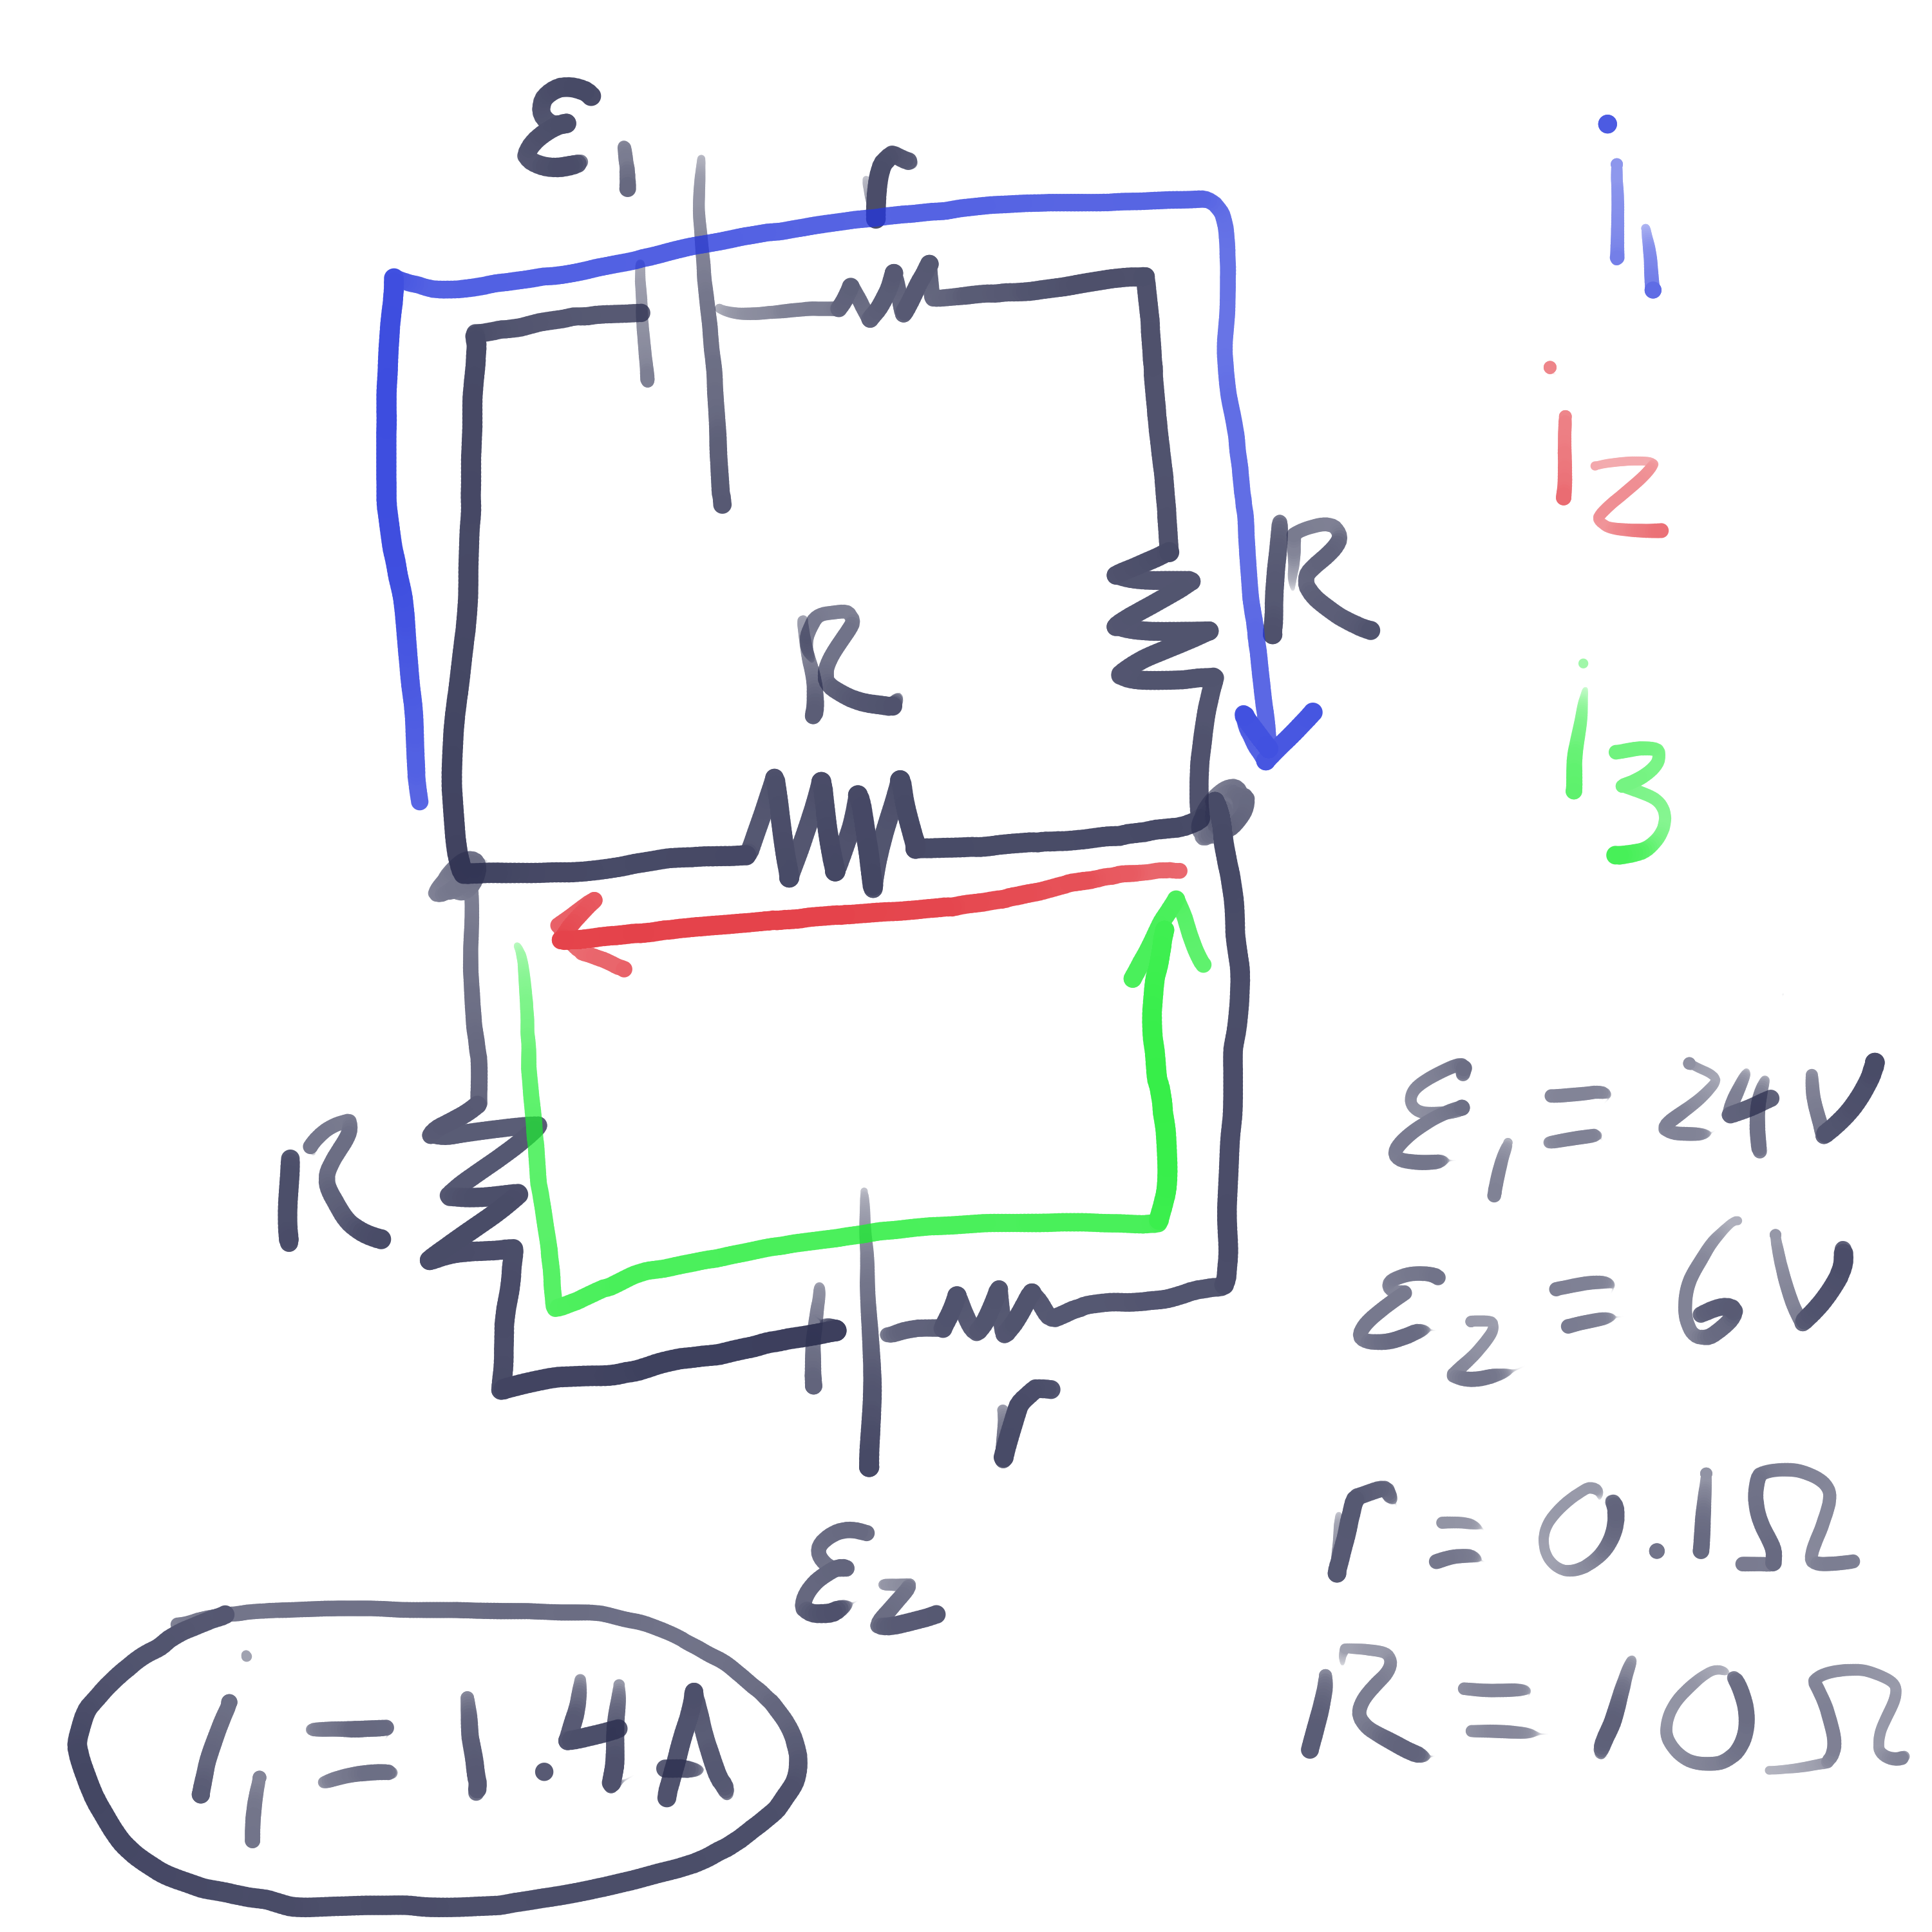
\includegraphics[width=0.4\textwidth]{kirchhoff_tutorial_circuit1.png}
\caption{\label{fig:dura} The circuit from Kirchhoff tutorial video 1.  Two batteries with internal resistances $r$ are connected to a circuit with resistors $R$.}
=======
\item $V = IR$ ... Ohm's Law
\item $R^{-1}_{\rm tot} = R_1^{-1} + R_2^{-1} + ...$ ... Adding resistors in parallel.
\item $R_{\rm tot} = R_1 + R_2 + ...$ ... Adding resistors in series.
\item $P = IV$ ... Power in DC circuits
\end{itemize}

\section{Complex Circuit}

\begin{enumerate}
\item (a) What is the total resistance in Fig. \ref{fig:dura}? (b) Find the current supplied by the source $V$. (c) Calculate the currents in each resistor and show that these add together to equal the current output of the source. (d) Calculate the power dissipated by each resistor. (e) Find the power output of the source and show that it equals the total power dissipated by the resistors.
\begin{figure}[ht]
\centering
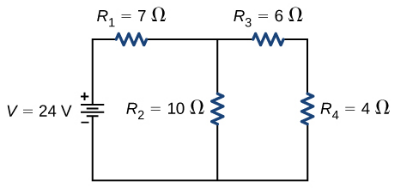
\includegraphics[width=0.5\textwidth]{circuit_series_parallel.png}
\caption{\label{fig:dura} A circuit involving four resistors.}
>>>>>>> 984fdb315abd4b8f89026c773978005f8f0c3ed8
\end{figure}
\end{enumerate}

\end{document}
